\section{Proposal}\label{sec:proposal}

\subsection{Requirements}

\subsubsection{Automation}



\subsubsection{Context-Awareness}

Applications may significantly differ in terms of the QoS they require from service providers. For example, autonomous vehicles may eventually rely on edge services for low-latency operations. An autonomous vehicle entering a given region for the first time is unlikely to be waiting until the edge servers covering that region become ready for providing the service the vehicle requires. 

Conversely, users of a mobile multiplayer game could eventually wait for a setup time whenever the edge servers nearby are not ready. In both cases, low-latency is an important requirement. However, the later type of application could afford a setup delay which the first could not. 

In addition, different kinds of edge infrastructure (e.g., more powerful servers or single board computers) or the same kind of edge infrastructure at different contexts (e.g., the number of clients in an area is too high in one region and low in another) may fit better with different policies for edge resources usage. Accordingly, the following requirement have been defined:

\textbf{R6:} Provisioning of edge resources must be context-dependent

\subsubsection{Heterogeneity, Discovery, and Selection}

An important aspect of edge computing consists of how the services provided by edge infrastructure should be discovered and consequently consumed by clients. 

Today, networking protocols and technologies are the main responsibles for allowing client applications to access cloud services in a transparent way. For this, clients access the services deployed in these datacenters by means of Internet names. 

Cloud datacenters are, at best, coarsely distributed among continents, countries, or regions. In these cases, service address are mapped to either the servers hosting them or to intermediate components (e.g., traffic managers) responsible for transparently routing client requests to datacenters covering their area. In contrast, in a fine grained geographical distribution of edge infrastructure, a similar transparency may not be possible. 

In particular, two scenarios of edge computing are possible: 1) edge servers are part of the telecommunications infrastructure (e.g., they are located at cellular base stations); 2) edge servers are part of conventional infrastructure  (e.g., they are located at malls, concert halls, stadiums, office buildings, parks, etc). 

In the first kind of scenario, which correspond to MEC, networking technology could be employed to make the decision of using edge or cloud infrastructure transparent for the client. For instance, active components at the base stations could divert the traffic coming from clients connected to that base station to local edge servers whenever the requested services are available or to the cloud otherwise~\cite{MEC_ROUTING}. 

Analogously, the second kind of scenario would require local network infrastructure components like access points and routers to actively divert the traffic from clients to edge servers in that location upon availability or to the cloud otherwise.

In both cases, clients requests would be transparently handled by either edge or cloud servers, with infrastructure components responsible for taking the edge-or-cloud decision. However, in the event of both types of edge infrastructure to coexist, the client would have to participate of an edge-or-edge kind of decision.

First, because it is unlikely that edge servers from different providers will be able to coordinate and decide which one will serve a given client request. For instance, at a given moment, a client device may be in contact with both MEC and indoor edge servers at an office building. If both can provide the same services, but are unable to coordinate among them, it is up to the client to decide which one to make use of. 

Second, because clients can switch from one network to the other at their discretion or make simultaneous use of different connections. For instance, once inside a building with some local edge servers accessible through Wi-Fi direct, the client may still decide for the edge server available at the base station it is connected (e.g., through 4G~\cite{4G}). As such, whereas independent edge servers would not see each other, the client would be able to see them and decide which one suits it the best.

In addition to the client participation in a edge-or-edge kind of decision, there is an argument in favor of giving the client also the responsibility for the edge-or-cloud type of decision: mobility. 

As mobile clients can enter or exit a given area, the less time a mobile client remains connected to a given edge server, the lower the chances of loosing connection before it is is still processing that client's request. Thus, if services are not currently available at local edge servers, clients should perform direct requests to the cloud and bypass any interaction with edge components. Fig. illustrates such scenario.

\begin{figure}
  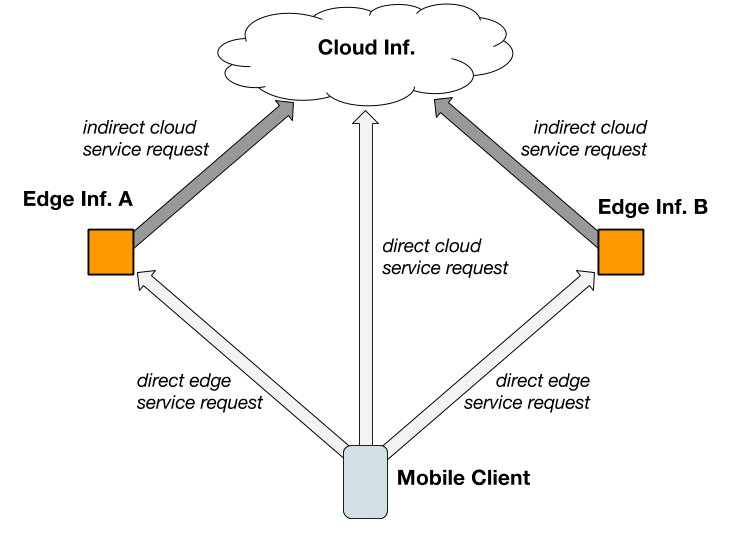
\includegraphics[width=0.7\textwidth]{figs/domain-selection.png}
  \caption{Two independent edge servers in range of communication with a client, which is responsible for choosing among one of these or the cloud; direct requests to the cloud eliminate the dependency with intermediary edge servers when they are unavailable}
  \label{fig:domain-selection}
\end{figure}


Thus, the client should be responsible for the decision of which alternative to use: the current best edge alternative, or the cloud. Once decided, the client-server interaction shall proceed without further ado.
Considering the points above, the following requirements have been elicited for the discovery and selection of different kinds of infrastructure:

\textbf{R1:} Edge infrastructure must be discoverable by clients; and 

\textbf{R2:} Clients must be able to choose among different independent alternatives of edge infrastructure and cloud infrastructure based on their requirements and the current state of the infrastructures they have access to.

TODO: replace R2 with: Control over forwarding from edge to cloud. Soft vs. strong constraint. Soft = I can also run on cloud if needed. Strong = Never go to cloud.

\subsubsection{Efficiency}

Another fundamental aspect of edge computing consists of how its highly distributed computational resources should be allocated to and consumed by different applications.

In cloud computing, the infrastructure responsible for hosting and performing services is abstracted away from client applications. The horizontal scalability cloud datacenters enable the optimization of services availability, i.e., cloud services should always be operational and accessible. ...in which backend applications are deployed to virtual machines and/or containers....

A direct replication of cloud computing IaaS model with edge infrastructure would not be possible. Instead, the fine grained nature of edge computing suggests the need of a different approach for the provisioning and usage of its computational resources. 

First, because it would mean that applications would have to be deployed to each edge server, even when there are no clients in the area been served. 
Second, because it is unlikely that a significant number of applications could be simultaneously hosted by edge infrastructure using technologies such as virtualization and containerization. 

Even if containers can be allocated faster than virtual machines~\cite{Giovanni}, at its best, a minumum amount of resources still needs to be allocated to each container. Thus, the scalability of edge computing in terms of number of simultaneous applications would be limited. 

Given the considerations above, the provisioning of edge infrastructure as a service can not simply mimic the model of IaaS employed with cloud computing. Accordingly, the following requirement for the allocation and usage of edge computational resources has been defined:
 
\textbf{R3:} Edge computational resources must be allocated on demand without minimum preallocation per application (opportunistic allocation) 
	
In addition to how edge resources should be allocated, the multiplicity of edge servers and their resource limitations also suggests that a priori deployment of different applications to all servers would impose unnecessary burden, as the assets of different applications would have to be acquired and stored independently of demand. Instead, to further optimize the usage of edge resources, the following requirement have been defined: 	

\textbf{R4:} Application resources must be acquired on demand (opportunistic acquisition) 

Finally, also considering the multiplicity of edge servers and the need for a scalable solution for the provisioning of edge infrastructure as a service, the following requirement have been defined:

\textbf{R5:} Application acquisition and allocation should be automated and not depend on  manual intervention from human administrators (self-management)
The fulfillment of the above requirements would leverage the potential of edge computing by optimizing the usage of its resources and consequently allowing a larger number of client applications to share the costs of edge infrastructure.

The resulting model would work as an extension of today’s cloud IaaS with the twofold purpose of enabling applications with low latency requirements to make use of edge infrastructure and to augment the computational power of mobile devices through mobile to edge computation offloading. 

\subsection{The A3-E Model}

To address the requirements R[1-6], we propose a unified model from which concrete models corresponding to different scenarios of edge computing can be instantiated. 
First, the interaction between potential clients and edge servers is decomposed into phases (Fig. 3). Each phase is characterized by some main activity from both sides. These activities are later refined with a flow diagram (Fig. 4). Finally, a reference architecture for the middlewares responsible for interfacing with client applications and edge servers is provided (Fig. 5).

From this point on, the term edge domain is used to abstract whatever computational resources can be employed by different edge providers at different sites. For instance, an edge domain could be composed of a grid of powerful servers at a cellular base station or a single cloudlet unit at some public event area. Also, it could be one or more single-board computer in a working office. It is also implied that edge domains are accessible by mobile clients through some (network) access point.

\begin{figure}
  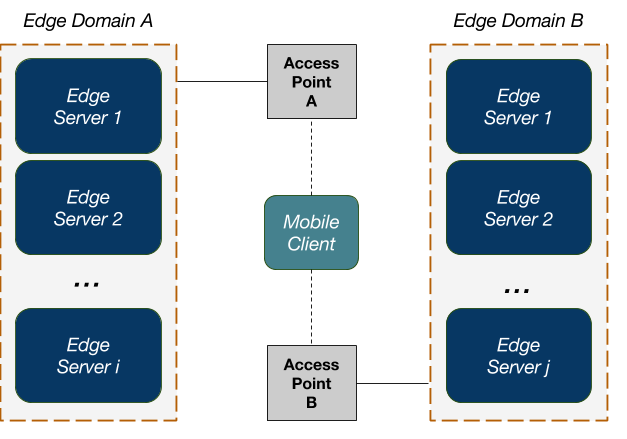
\includegraphics[width=0.5\textwidth]{figs/edge-domain-client.png}
  \caption{Computational resources abstracted under different edge domains; a mobile client within connection range to edge domains A and B through access points A and B}
  \label{fig:edge-domain-client}
\end{figure}

\subsubsection{A3-E: Phases}

\begin{figure}[htbp]
	\centering
	\captionsetup[subfigure]{width=\textwidth}
	\subfloat[Different phases of the A3-E model; phases are delimited by vertical lines and the main activities by inner labels in both clients and domains; labeled oval shapes represent the respective states of both sides at the end of each phase\label{fig:cloud-to-edge}]{ 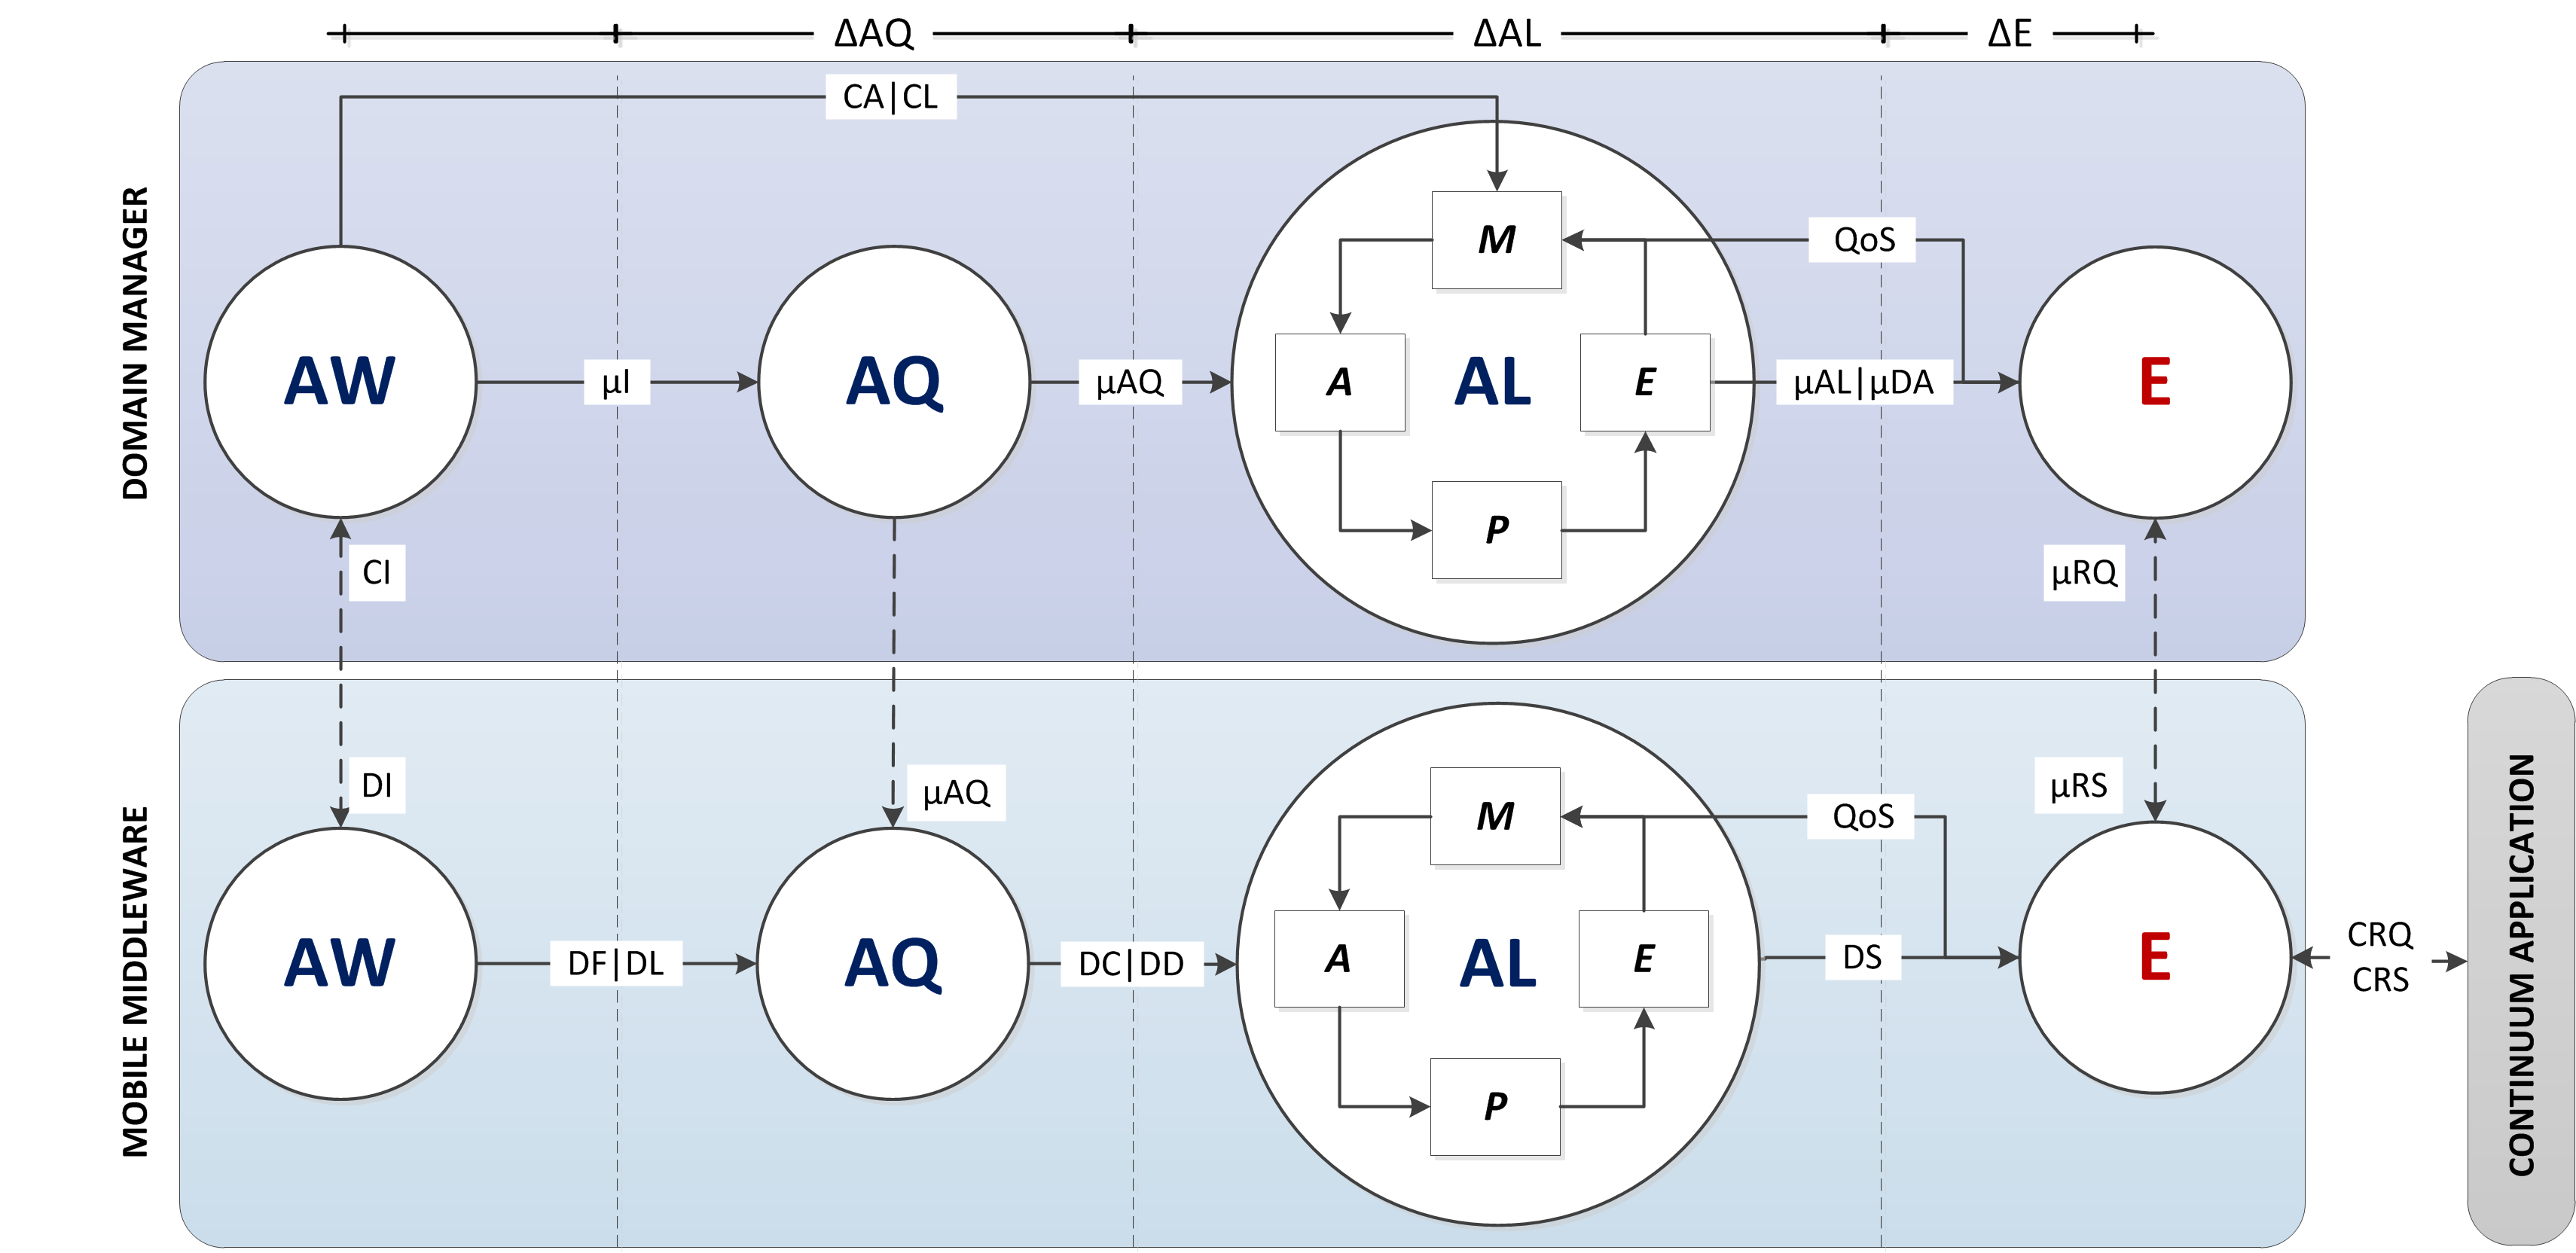
\includegraphics[width=0.9\textwidth]{figs/A3-E.png}}\hfill
	
	\raggedright
	\subfloat[Different states of a given edge domain with respect to a given client application; the transitions between states triggered by domain events are guarded by policies that may vary according to the type of edge infrastructure and application\label{fig:A3-E-domain}] {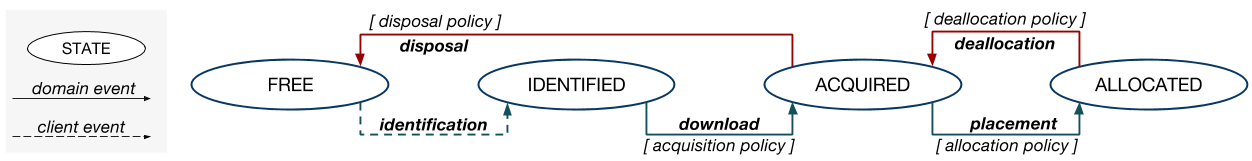
\includegraphics[width=0.95\textwidth]{figs/A3-E-domain.png}}\hfill
	
	\subfloat[Different states of a given client with respect to a given edge domain; the transitions between states triggered by client events are guarded by policies that may vary according to the client requirements\label{fig:A3-E-client}] {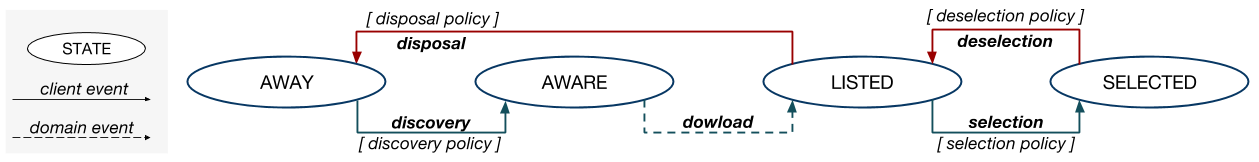
\includegraphics[width=0.95\textwidth]{figs/A3-E-client.png}}\hfill
	\caption{The A3-E Model} \label{fig:1}
\end{figure}


%\begin{figure}
%  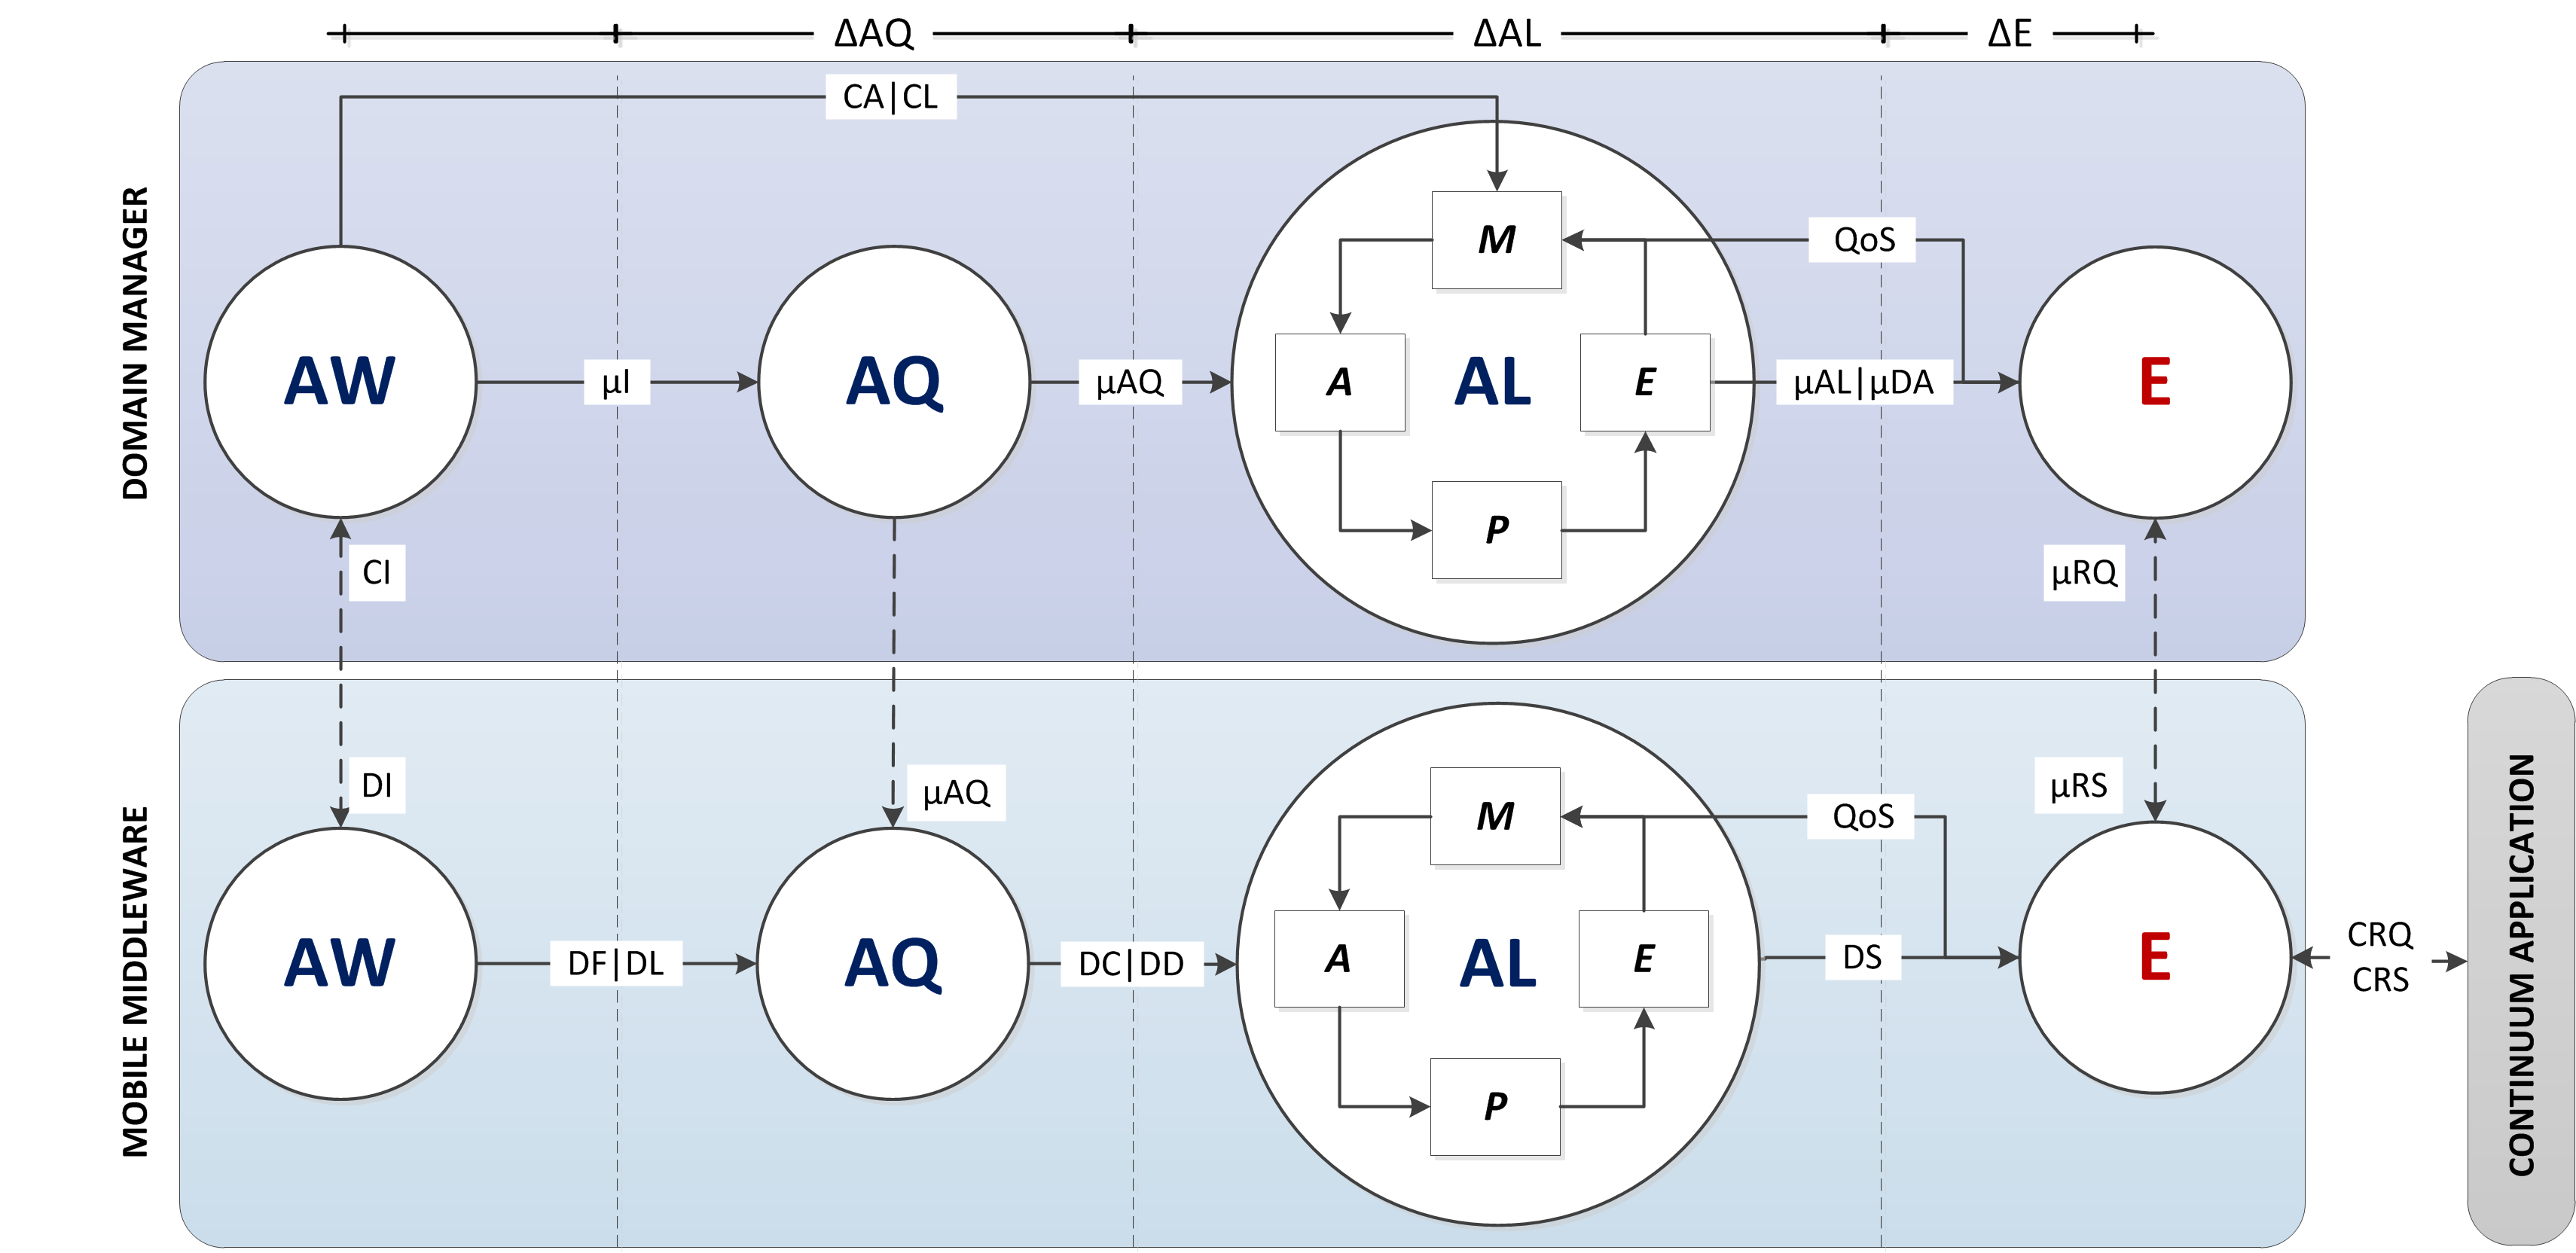
\includegraphics[width=0.9\textwidth]{figs/A3-E.png}
%  \caption{Different phases of the A3-E model; phases are delimited by vertical lines and the main activities by inner labels in both clients and domains; labeled oval shapes represent the respective states of both sides at the end of each phase}
%  \label{fig:A3-E}
%\end{figure}
%
%\begin{figure}
%  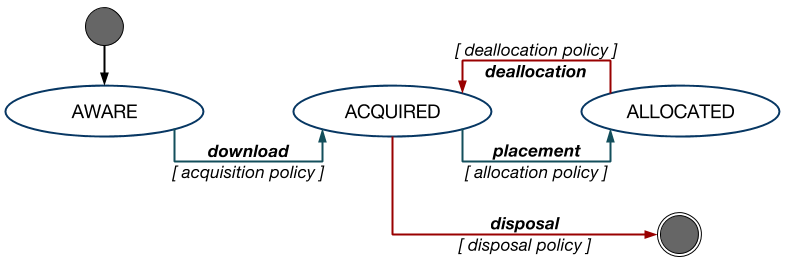
\includegraphics[width=0.95\textwidth]{figs/A3-E-states.png}
%  \caption{Different states of a given edge domain with respect to a given application; the transitions between awareness, acquisition, and allocation are guarded by policies that may vary according to the type of application and to the type of edge infrastructure}
%  \label{fig:states}
%\end{figure}

The diagram in Fig. 3 captures the different phases of the interaction between a mobile client running a given application that first contacts a given edge domain. 
	
In accordance with requirement R1, edge domains perform the advertisement of their existence to whatever clients may be in reach. Potential clients, in their turn, must perform the discovery of edge domains. Before a given domain is found, it remains unknown to that client.

To address requirement R3 and R4, edge domains must remain free with respect to some application until the contact with a potential mobile client hosting that application. This condition refers to both the storage of application assets (e.g., code, libraries, etc), as well as the allocation of these assets for execution (e.g., deployment and instantiation of a restful application). 

Once a given domain has been discovered, the client must proceed with the identification of the application it is running. This process enables the edge domain to download whatever assets required by that specific application.  

The acquisition of application components does not make them ready to be executed. Instead, valuable resources like memory and CPU are kept free w.r.t. this application until the domain proceed with the placement of the application components as part of the allocation phase. The later activity corresponds to the allocation of resources from one or more domain servers required for the application execution. 	

Finally, once the allocation phase is finished, the domain is ready to perform the computation required by the application. For instance, following a request-response protocol, clients can fire requisitions to that domain. These activities are part of the engagement phase.

The separation of phases emphasizes not only the different concerns involved, but also the distinction between the moments they occur. The transition among phases may either be sequential, meaning that one phase starts as soon the previous finishes, or conditional, meaning that additional condition(s) must be met before the next phase can start. 	

Fig. x presents the possible transitions among the three A phases of an edge domain regarding a given application. The awareness-acquisition transition is modelled by three alternative policies: 

\begin{itemize}

\item proactive acquisition: phase starts as soon as the edge domain becomes active; 

\item partially proactive acquisition: phase starts as soon as awareness phase finishes; or

\item reactive acquisition: phase starts as soon as awareness phase finishes and the client notifies its intention for using that domain.

\end{itemize}

The acquisition-allocation transition, in its turn, is modelled by two alternative policies: 

\begin{itemize}

\item proactive allocation: phase starts as soon as acquisition phase finishes; or

\item reactive allocation: phase starts as soon as acquisition phase finishes and the client notifies its intention for using that domain.

\end{itemize}

Finally, reverse transitions are single and dependent on the specific policies for deallocating and disposing of application assets. 
In accordance with Requirement R6, the aforementioned policies are useful for different classes of applications, as well as different types of edge computing infrastructure and different usage contexts.


TODO: discuss below how each of the aforementioned policies address specific requirements elicited in the previous section; pros-cons

\subsection{A3-E: Refined Activities}

\begin{figure}
  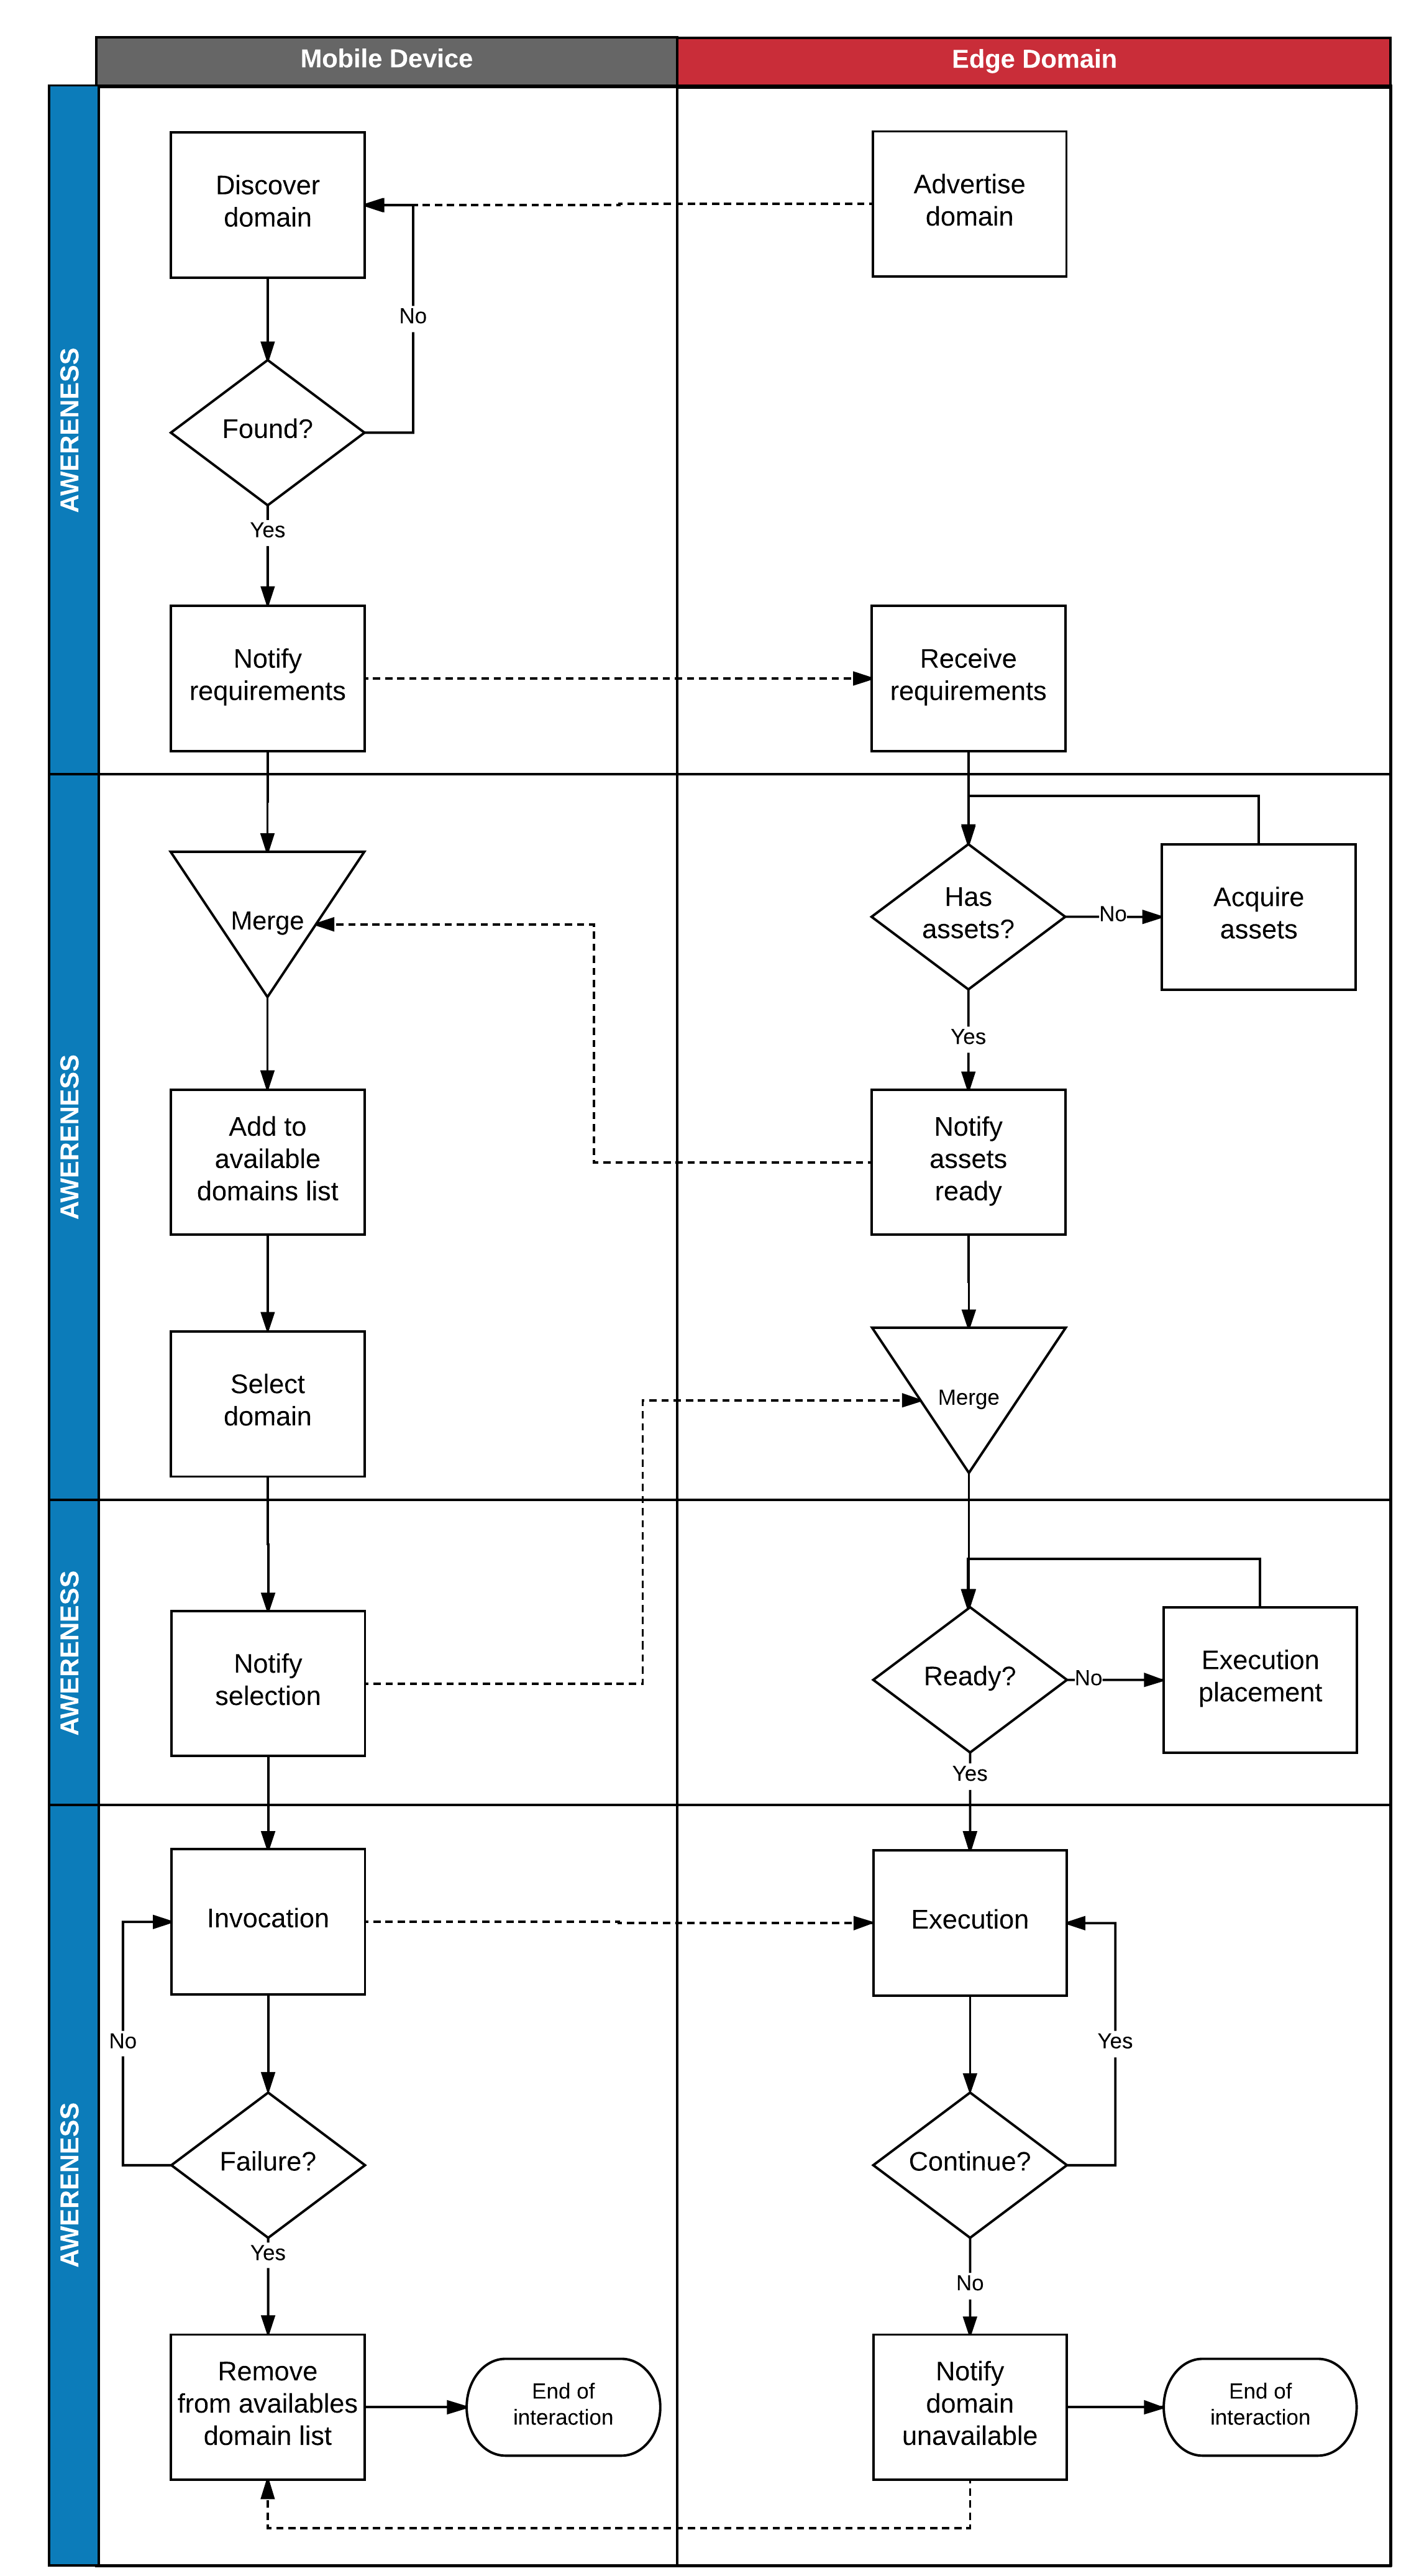
\includegraphics[height=\textheight]{figs/activities.png}
  \caption{TODO}
  \label{fig:activities}
\end{figure}

\subsection{A3-E: Reference Architecture}

\begin{figure}
  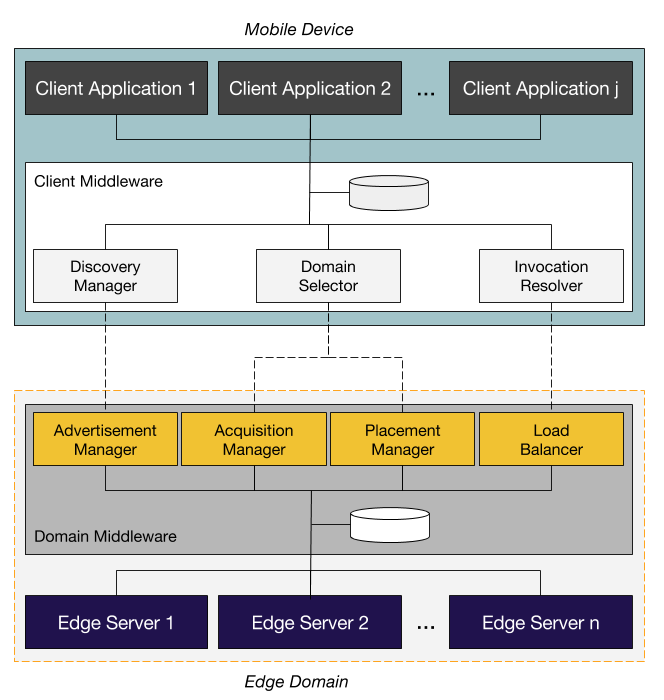
\includegraphics[width=0.6\textwidth]{figs/reference-architecture.png}
  \caption{TODO}
  \label{fig:reference-architecture}
\end{figure}

%the client applications hosted by a mobile devices interact with a domain through a client middleware; the domain has its own middleware responsible for the activities in the A3-E model and interfaces with the servers in that domain


\subsection{A3-E: Protocols}

\begin{figure}
  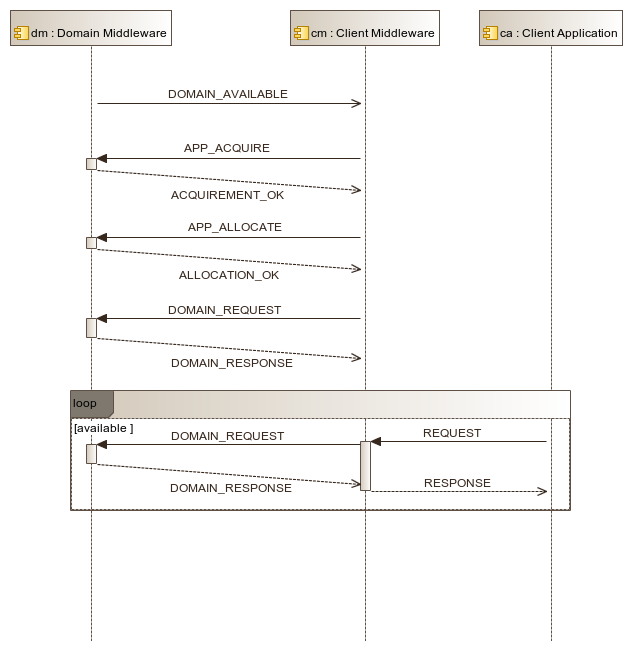
\includegraphics[width=0.6\textwidth]{figs/protocols.png}
  \caption{TODO}
  \label{fig:protocols}
\end{figure}
